\documentclass{article}

\usepackage{tikz}
\usepackage{amsmath}
\usetikzlibrary{matrix}
\usetikzlibrary {shapes.geometric}
\usetikzlibrary {positioning}
\usetikzlibrary {decorations.pathmorphing}
\usetikzlibrary {arrows.meta}

\usepackage{hyperref}

\begin{document}
    \title{HBots}
    \author{Daniel de la Cruz Prieto} 

    \maketitle

    \begin{abstract}
        \noindent En este articulos vamos resolver el el problema H.Bots de juez en linea COJ. 
        Se hace en anilisas de las vias de soluciones que tiene el problema , se lleva 
        al lenguaje tecnico de Matematica Discreta para dar respuesta a al mismo usando 
        resultados de Teor\'ia de N\'umeros y combinatoria vistos en clase   
    \end{abstract}


    \section{Orden del Problema} 

    \section{An\'alisis del Problema } 

    \section{Solucion del Problema } 
    \section{Correctitud del Algoritmo} 
    \section{Complejidad temporal del algoritmo} 

    \newpage

    \begin{center}
        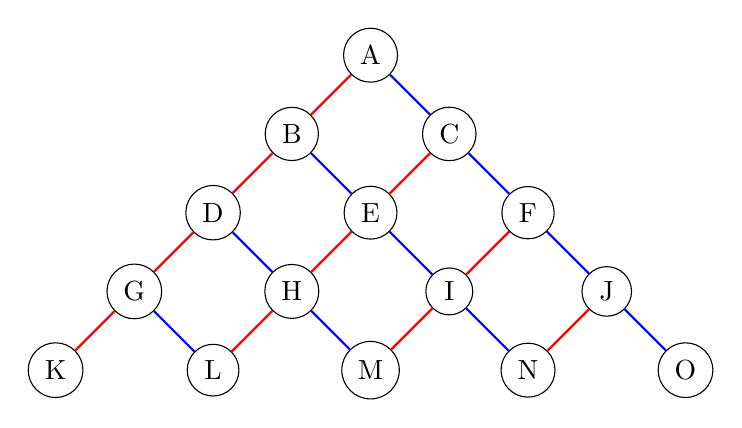
\begin{tikzpicture}

            %\draw [help lines] (0,0) grid (10,10); 

            \path   (5,10)  node (a) [circle,draw] {A}
                    (4,9) node (b) [circle,draw] {B}
                    (6,9) node (c) [circle,draw] {C}
                    (3,8) node (d) [circle,draw] {D}
                    (5,8) node (e) [circle,draw] {E}
                    (7,8) node (f) [circle,draw] {F}
                    (2,7) node (g) [circle,draw] {G}
                    (4,7) node (h) [circle,draw] {H}
                    (6,7) node (i) [circle,draw] {I}
                    (8,7) node (j) [circle,draw] {J}
                    (1,6) node (k) [circle,draw] {K}
                    (3,6) node (l) [circle,draw] {L}
                    (5,6) node (m) [circle,draw] {M}
                    (7,6) node (n) [circle,draw] {N}
                    (9,6) node (o) [circle,draw] {O};
                
            \draw[thick,red]  (node cs: name =a ) -- (node cs:name =b);
            \draw[thick,blue] (node cs: name =a ) -- (node cs:name =c);
            \draw[thick,red] (node cs: name =b ) -- (node cs:name =d);
            \draw[thick,blue] (node cs: name =b ) -- (node cs:name =e);
            \draw[thick,red] (node cs: name =d ) -- (node cs:name =g);
            \draw[thick,red] (node cs: name =c ) -- (node cs:name =e);
            \draw[thick,blue] (node cs: name =c ) -- (node cs:name =f);
            \draw[thick,red] (node cs: name =g ) -- (node cs:name =k);
            \draw[thick,blue] (node cs: name =g ) -- (node cs:name =l);
            \draw[thick,blue] (node cs: name =d ) -- (node cs:name =h);
            \draw[thick,red] (node cs: name =h ) -- (node cs:name =l);
            \draw[thick,red] (node cs: name =e ) -- (node cs:name =h);
            \draw[thick,blue] (node cs: name =h ) -- (node cs:name =m);
            \draw[thick,blue] (node cs: name =e ) -- (node cs:name =i);
            \draw[thick,red] (node cs: name =i ) -- (node cs:name =m);
            \draw[thick,blue] (node cs: name =i ) -- (node cs:name =n);
            \draw[thick,red] (node cs: name =f ) -- (node cs:name =i);
            \draw[thick,blue] (node cs: name =f ) -- (node cs:name =j);
            \draw[thick,red] (node cs: name =j ) -- (node cs:name =n);
            \draw[thick,blue] (node cs: name =j ) -- (node cs:name =o);
        \end{tikzpicture}
    \end{center}

    \newpage

    \begin{center}
        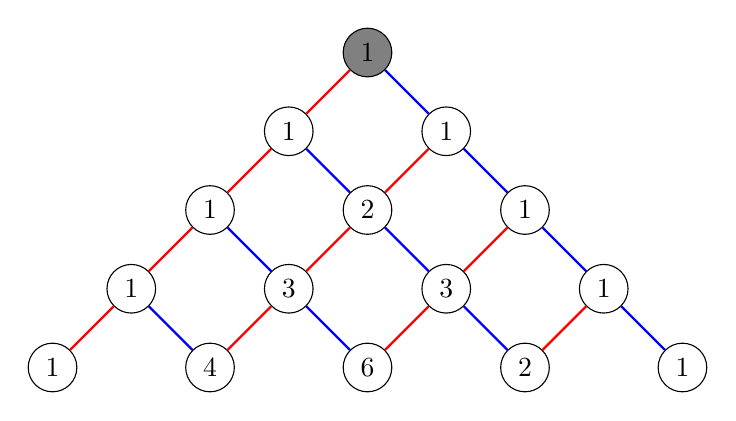
\begin{tikzpicture}

            %\draw [help lines] (0,0) grid (10,10); 

            \path   (5,10)  node (a) [circle,draw,fill = gray] {1}
                    (4,9) node (b) [circle,draw] {1}
                    (6,9) node (c) [circle,draw] {1}
                    (3,8) node (d) [circle,draw] {1}
                    (5,8) node (e) [circle,draw] {2}
                    (7,8) node (f) [circle,draw] {1}
                    (2,7) node (g) [circle,draw] {1}
                    (4,7) node (h) [circle,draw] {3}
                    (6,7) node (i) [circle,draw] {3}
                    (8,7) node (j) [circle,draw] {1}
                    (1,6) node (k) [circle,draw] {1}
                    (3,6) node (l) [circle,draw] {4}
                    (5,6) node (m) [circle,draw] {6}
                    (7,6) node (n) [circle,draw] {2}
                    (9,6) node (o) [circle,draw] {1};
                
            \draw[thick,red]  (node cs: name =a ) -- (node cs:name =b);
            \draw[thick,blue] (node cs: name =a ) -- (node cs:name =c);
            \draw[thick,red] (node cs: name =b ) -- (node cs:name =d);
            \draw[thick,blue] (node cs: name =b ) -- (node cs:name =e);
            \draw[thick,red] (node cs: name =d ) -- (node cs:name =g);
            \draw[thick,red] (node cs: name =c ) -- (node cs:name =e);
            \draw[thick,blue] (node cs: name =c ) -- (node cs:name =f);
            \draw[thick,red] (node cs: name =g ) -- (node cs:name =k);
            \draw[thick,blue] (node cs: name =g ) -- (node cs:name =l);
            \draw[thick,blue] (node cs: name =d ) -- (node cs:name =h);
            \draw[thick,red] (node cs: name =h ) -- (node cs:name =l);
            \draw[thick,red] (node cs: name =e ) -- (node cs:name =h);
            \draw[thick,blue] (node cs: name =h ) -- (node cs:name =m);
            \draw[thick,blue] (node cs: name =e ) -- (node cs:name =i);
            \draw[thick,red] (node cs: name =i ) -- (node cs:name =m);
            \draw[thick,blue] (node cs: name =i ) -- (node cs:name =n);
            \draw[thick,red] (node cs: name =f ) -- (node cs:name =i);
            \draw[thick,blue] (node cs: name =f ) -- (node cs:name =j);
            \draw[thick,red] (node cs: name =j ) -- (node cs:name =n);
            \draw[thick,blue] (node cs: name =j ) -- (node cs:name =o);
        \end{tikzpicture}
    \end{center}
   

    \newpage

    \begin{center}
        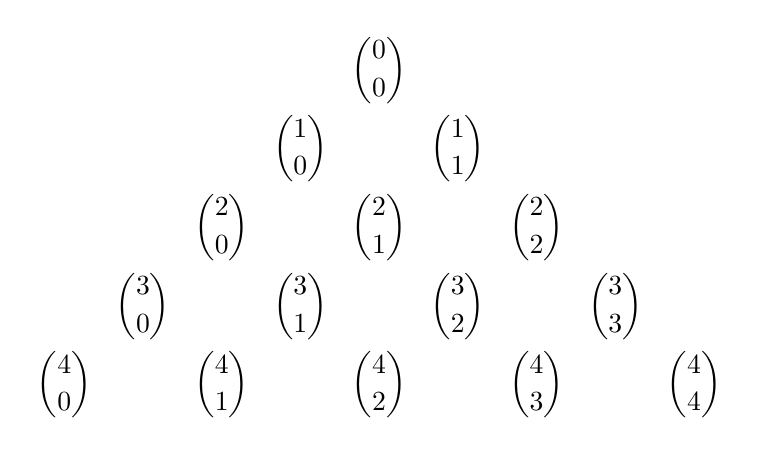
\begin{tikzpicture}

            %\draw [help lines] (0,0) grid (10,10); 

            \path   (5,10) node (a) [] {\mbox{$\displaystyle \binom{0}{0}$ }}
                    (4,9) node (b) [] {\mbox{$\displaystyle \binom{1}{0}$ }}
                    (6,9) node (c) [] {\mbox{$\displaystyle \binom{1}{1}$ }}
                    (3,8) node (d) [] {\mbox{$\displaystyle \binom{2}{0}$ }}
                    (5,8) node (e) [] {\mbox{$\displaystyle \binom{2}{1}$ }}
                    (7,8) node (f) [] {\mbox{$\displaystyle \binom{2}{2}$ }}
                    (2,7) node (g) [] {\mbox{$\displaystyle \binom{3}{0}$ }}
                    (4,7) node (h) [] {\mbox{$\displaystyle \binom{3}{1}$ }}
                    (6,7) node (i) [] {\mbox{$\displaystyle \binom{3}{2}$ }}
                    (8,7) node (j) [] {\mbox{$\displaystyle \binom{3}{3}$ }}
                    (1,6) node (k) [] {\mbox{$\displaystyle \binom{4}{0}$ }}
                    (3,6) node (l) [] {\mbox{$\displaystyle \binom{4}{1}$ }}
                    (5,6) node (m) [] {\mbox{$\displaystyle \binom{4}{2}$ }}
                    (7,6) node (n) [] {\mbox{$\displaystyle \binom{4}{3}$ }}
                    (9,6) node (o) [] {\mbox{$\displaystyle \binom{4}{4}$ }};
                
            % \draw[thick,red]  (node cs: name =a ) -- (node cs:name =b);
            % \draw[thick,blue] (node cs: name =a ) -- (node cs:name =c);
            % \draw[thick,red] (node cs: name =b ) -- (node cs:name =d);
            % \draw[thick,blue] (node cs: name =b ) -- (node cs:name =e);
            % \draw[thick,red] (node cs: name =d ) -- (node cs:name =g);
            % \draw[thick,red] (node cs: name =c ) -- (node cs:name =e);
            % \draw[thick,blue] (node cs: name =c ) -- (node cs:name =f);
            % \draw[thick,red] (node cs: name =g ) -- (node cs:name =k);
            % \draw[thick,blue] (node cs: name =g ) -- (node cs:name =l);
            % \draw[thick,blue] (node cs: name =d ) -- (node cs:name =h);
            % \draw[thick,red] (node cs: name =h ) -- (node cs:name =l);
            % \draw[thick,red] (node cs: name =e ) -- (node cs:name =h);
            % \draw[thick,blue] (node cs: name =h ) -- (node cs:name =m);
            % \draw[thick,blue] (node cs: name =e ) -- (node cs:name =i);
            % \draw[thick,red] (node cs: name =i ) -- (node cs:name =m);
            % \draw[thick,blue] (node cs: name =i ) -- (node cs:name =n);
            % \draw[thick,red] (node cs: name =f ) -- (node cs:name =i);
            % \draw[thick,blue] (node cs: name =f ) -- (node cs:name =j);
            % \draw[thick,red] (node cs: name =j ) -- (node cs:name =n);
            % \draw[thick,blue] (node cs: name =j ) -- (node cs:name =o);
        \end{tikzpicture}

    \end{center}

    \newpage

    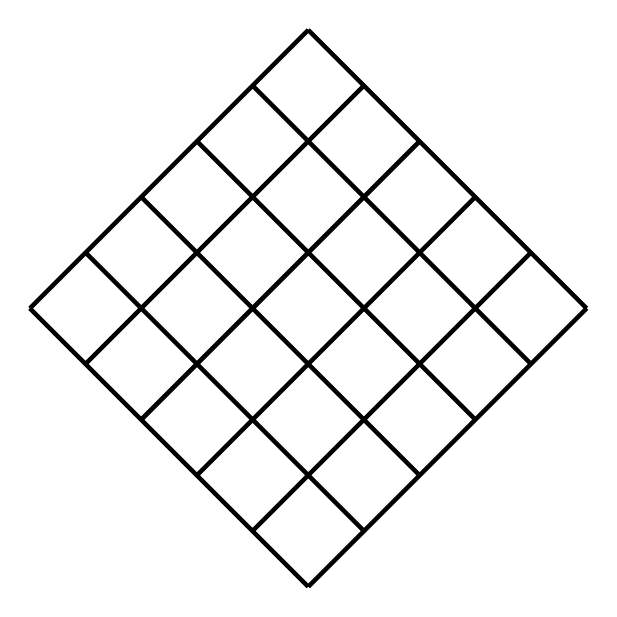
\begin{tikzpicture}
        %\draw [help lines] (0,0) grid (10,10); 
        \draw[step= 1cm,gray,ultra thick , color = black ,rotate = 45] (0,0) grid (5,5);
    \end{tikzpicture}



    \newpage
    
%Figura del TURNO 2 
    \begin{center}
        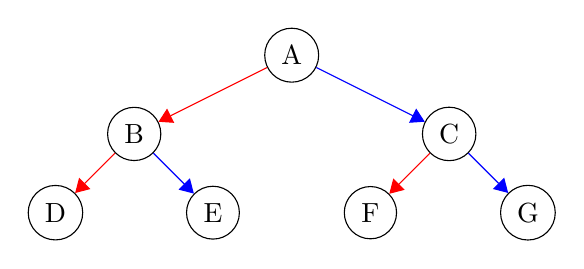
\begin{tikzpicture}

            %\draw [help lines] (0,0) grid (10,10); 

            \path   (5,10)  node (a) [circle,draw] {A}
                    (3,9) node (b) [circle,draw] {B}
                    (7,9) node (c) [circle,draw] {C}
                    (2,8) node (d) [circle,draw] {D}
                    (4,8) node (e) [circle,draw] {E}
                    (6,8) node (f) [circle,draw] {F}
                    (8,8) node (g) [circle,draw] {G};
                    
                
            \draw[arrows = -{Triangle[open,angle=60:2mm,fill = red]},red]  (node cs: name =a ) -- (node cs:name =b);
            \draw[arrows = -{Triangle[open,angle=60:2mm,fill = blue]},blue] (node cs: name =a ) -- (node cs:name =c);
            \draw[arrows = -{Triangle[open,angle=60:2mm,fill = red]},red] (node cs: name =b ) -- (node cs:name =d);
            \draw[arrows = -{Triangle[open,angle=60:2mm,fill = blue]},blue] (node cs: name =b ) -- (node cs:name =e);
            \draw[arrows = -{Triangle[open,angle=60:2mm,fill = red]},red] (node cs: name =c ) -- (node cs:name =f);
            \draw[arrows = -{Triangle[open,angle=60:2mm,fill = blue]},blue] (node cs: name =c ) -- (node cs:name =g);
            
        \end{tikzpicture}
    \end{center}

    \newpage

    \subsection*{Turno 3}
    %TURNO 3 
    \begin{center}
        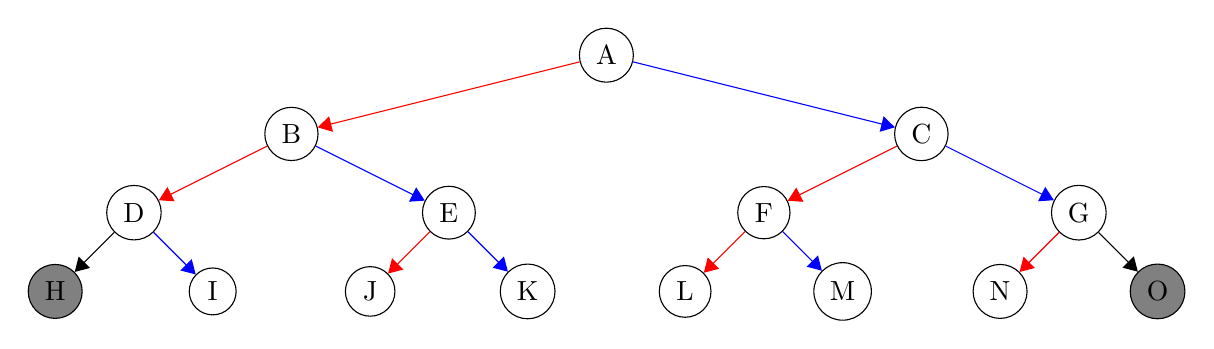
\begin{tikzpicture}

            %\draw [help lines] (0,0) grid (16,16); 

            \path   (8,10)  node (a) [circle,draw] {A}
                    (4,9) node (b) [circle,draw] {B}
                    (12,9) node (c) [circle,draw] {C}
                    (2,8) node (d) [circle,draw] {D}
                    (6,8) node (e) [circle,draw] {E}
                    (10,8) node (f) [circle,draw] {F}
                    (14,8) node (g) [circle,draw] {G}
                    (1,7) node (h) [circle,draw,fill=gray] {H}
                    (3,7) node (i) [circle,draw] {I}
                    (5,7) node (j) [circle,draw] {J}
                    (7,7) node (k) [circle,draw] {K}
                    (9,7) node (l) [circle,draw] {L}
                    (11,7) node (m) [circle,draw] {M}
                    (13,7) node (n) [circle,draw] {N}
                    (15,7) node (o) [circle,draw,fill = gray] {O};

                    
                
            \draw[arrows = -{Triangle[open,angle=60:2mm,fill = red]},red]  (node cs: name =a ) -- (node cs:name =b);
            \draw[arrows = -{Triangle[open,angle=60:2mm,fill = blue]},blue] (node cs: name =a ) -- (node cs:name =c);
            \draw[arrows = -{Triangle[open,angle=60:2mm,fill = red]},red] (node cs: name =b ) -- (node cs:name =d);
            \draw[arrows = -{Triangle[open,angle=60:2mm,fill = blue]},blue] (node cs: name =b ) -- (node cs:name =e);
            \draw[arrows = -{Triangle[open,angle=60:2mm,fill = red]},red] (node cs: name =c ) -- (node cs:name =f);
            \draw[arrows = -{Triangle[open,angle=60:2mm,fill = blue]},blue] (node cs: name =c ) -- (node cs:name =g);
            \draw[arrows = -{Triangle[open,angle=60:2mm,fill = black]},black] (node cs: name =d ) -- (node cs:name =h);
            \draw[arrows = -{Triangle[open,angle=60:2mm,fill = red]},red] (node cs: name =e ) -- (node cs:name =j);
            \draw[arrows = -{Triangle[open,angle=60:2mm,fill = red]},red] (node cs: name =f ) -- (node cs:name =l);
            \draw[arrows = -{Triangle[open,angle=60:2mm,fill = red]},red] (node cs: name =g) -- (node cs:name =n);
            \draw[arrows = -{Triangle[open,angle=60:2mm,fill = blue]},blue] (node cs: name =d ) -- (node cs:name =i);
            \draw[arrows = -{Triangle[open,angle=60:2mm,fill = blue]},blue] (node cs: name =e ) -- (node cs:name =k);
            \draw[arrows = -{Triangle[open,angle=60:2mm,fill = blue]},blue] (node cs: name =f) -- (node cs:name =m);
            \draw[arrows = -{Triangle[open,angle=60:2mm,fill = black]},black] (node cs: name =g ) -- (node cs:name =o);
            
        \end{tikzpicture}
    \end{center}

    \newpage

    \subsubsection*{Turno 3.1}
    %Turno 3
    \begin{center}
        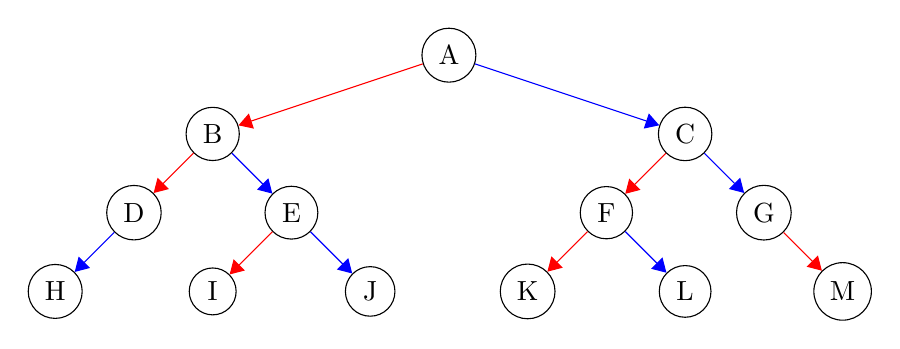
\begin{tikzpicture}

            %\draw [help lines] (0,0) grid (16,16); 

            \path   (8,10)  node (a) [circle,draw] {A}
                    (5,9) node (b) [circle,draw] {B}
                    (11,9) node (c) [circle,draw] {C}
                    (4,8) node (d) [circle,draw] {D}
                    (6,8) node (e) [circle,draw] {E}
                    (10,8) node (f) [circle,draw] {F}
                    (12,8) node (g) [circle,draw] {G}
                    (3,7) node (h) [circle,draw] {H}
                    (5,7) node (i) [circle,draw] {I}
                    (7,7) node (j) [circle,draw] {J}
                    (9,7) node (k) [circle,draw] {K}
                    (11,7) node (l) [circle,draw] {L}
                    (13,7) node (m) [circle,draw] {M};
                    %(13,7) node (n) [circle,draw] {N}
                    %(15,7) node (o) [circle,draw] {O};

                    
                
            \draw[arrows = -{Triangle[open,angle=60:2mm,fill = red]},red]  (node cs: name =a ) -- (node cs:name =b);
            \draw[arrows = -{Triangle[open,angle=60:2mm,fill = blue]},blue] (node cs: name =a ) -- (node cs:name =c);
            \draw[arrows = -{Triangle[open,angle=60:2mm,fill = red]},red] (node cs: name =b ) -- (node cs:name =d);
            \draw[arrows = -{Triangle[open,angle=60:2mm,fill = blue]},blue] (node cs: name =b ) -- (node cs:name =e);
            \draw[arrows = -{Triangle[open,angle=60:2mm,fill = red]},red] (node cs: name =c ) -- (node cs:name =f);
            \draw[arrows = -{Triangle[open,angle=60:2mm,fill = blue]},blue] (node cs: name =c ) -- (node cs:name =g);
            \draw[arrows = -{Triangle[open,angle=60:2mm,fill = blue]},blue] (node cs: name =d ) -- (node cs:name =h);
            \draw[arrows = -{Triangle[open,angle=60:2mm,fill = red]},red] (node cs: name =e ) -- (node cs:name =i);
            \draw[arrows = -{Triangle[open,angle=60:2mm,fill = blue]},blue] (node cs: name =e ) -- (node cs:name =j);
            \draw[arrows = -{Triangle[open,angle=60:2mm,fill = red]},red] (node cs: name =f) -- (node cs:name =k);
            \draw[arrows = -{Triangle[open,angle=60:2mm,fill = blue]},blue] (node cs: name =f ) -- (node cs:name =l);
            \draw[arrows = -{Triangle[open,angle=60:2mm,fill = red]},red] (node cs: name =g ) -- (node cs:name =m);
            %\draw[thick,blue] (node cs: name =f) -- (node cs:name =m);
            %\draw[thick,black] (node cs: name =g ) -- (node cs:name =o);
            
        \end{tikzpicture}
    \end{center}

    \newpage

    \begin{center}
        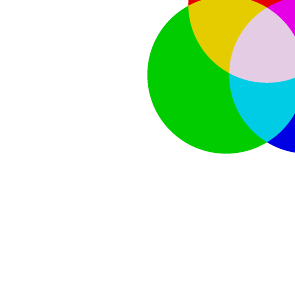
\begin{tikzpicture}
            \tikz [transparency group]
            {
            \pgfsetblendmode{screen}

            \fill[red!90!black]( 90:.6) circle (1);
            \fill[green!80!black] (210:.6) circle (1);
            \fill[blue!90!black] (330:.6) circle (1);
            }
        \end{tikzpicture}
    \end{center}
    
    \newpage
    
    \begin{center}
        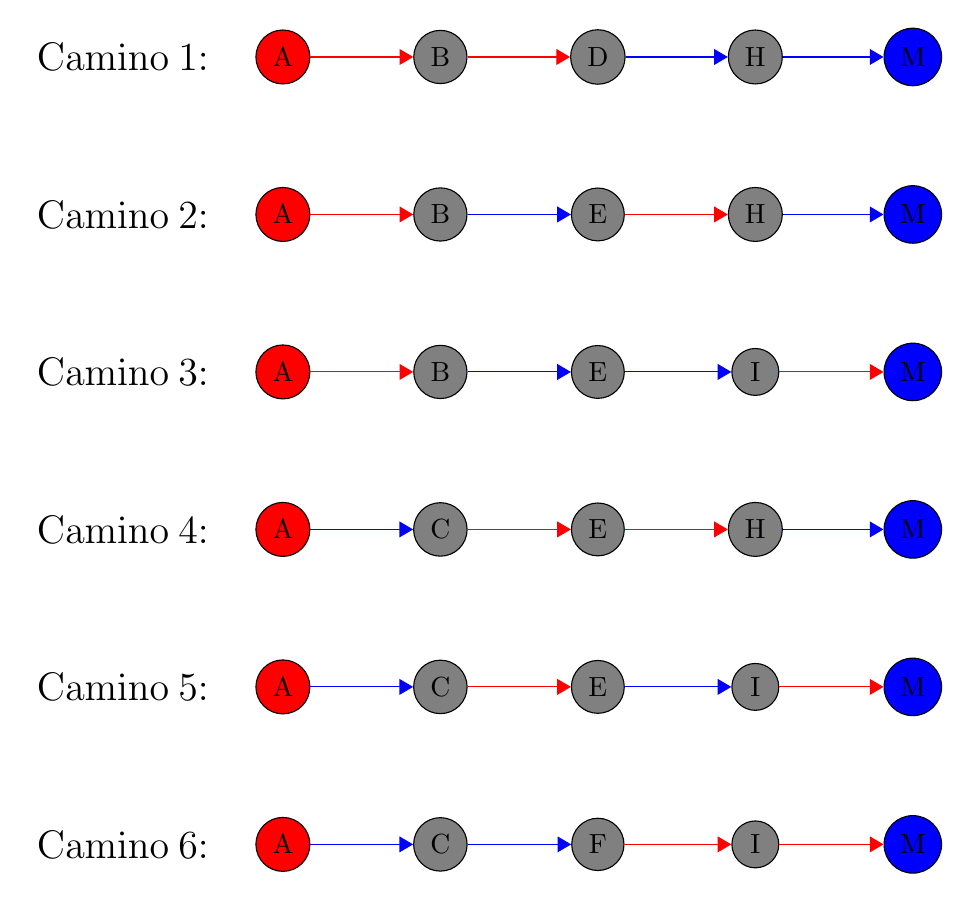
\begin{tikzpicture}

            % \draw [help lines] (0,0) grid (8,12); 

            \path   (0,10) node (a) [circle,draw,fill=red] {A}
                    (2,10) node (b) [circle,draw,fill=gray] {B}
                    (4,10) node (c) [circle,draw,fill=gray] {D}
                    (6,10) node (d) [circle,draw,fill=gray] {H}
                    (8,10) node (e) [circle,draw,fill=blue] {M}
                    
                    (0,8) node (f) [circle,draw,fill=red] {A}
                    (2,8) node (g) [circle,draw,fill=gray] {B}
                    (4,8) node (h) [circle,draw,fill=gray] {E}
                    (6,8) node (i) [circle,draw,fill=gray] {H}
                    (8,8) node (j) [circle,draw,fill=blue] {M}

                    (0,6) node (k) [circle,draw,fill=red] {A}
                    (2,6) node (l) [circle,draw,fill=gray] {B}
                    (4,6) node (m) [circle,draw,fill=gray] {E}
                    (6,6) node (n) [circle,draw,fill=gray] {I}
                    (8,6) node (o) [circle,draw,fill=blue] {M}

                    (0,4) node (p) [circle,draw,fill=red] {A}
                    (2,4) node (q) [circle,draw,fill=gray] {C}
                    (4,4) node (r) [circle,draw,fill=gray] {E}
                    (6,4) node (s) [circle,draw,fill=gray] {H}
                    (8,4) node (t) [circle,draw,fill=blue] {M}

                    (0,2) node (u) [circle,draw,fill=red] {A}
                    (2,2) node (v) [circle,draw,fill=gray] {C}
                    (4,2) node (w) [circle,draw,fill=gray] {E}
                    (6,2) node (x) [circle,draw,fill=gray] {I}
                    (8,2) node (y) [circle,draw,fill=blue] {M}

                    (0,0) node (uz) [circle,draw,fill=red] {A}
                    (2,0) node (vz) [circle,draw,fill=gray] {C}
                    (4,0) node (wz) [circle,draw,fill=gray] {F}
                    (6,0) node (xz) [circle,draw,fill=gray] {I}
                    (8,0) node (yz) [circle,draw,fill=blue] {M};
                    




                    
                
            \draw[arrows = -{Triangle[open, angle=60:2mm,fill=red]},red] (node cs: name =a ) -- (node cs:name =b);
            \draw[arrows = -{Triangle[open, angle=60:2mm,fill=red]},red] (node cs: name =b ) -- (node cs:name =c);
            \draw[arrows = -{Triangle[open, angle=60:2mm,fill=blue]},blue] (node cs: name =c ) -- (node cs:name =d);
            \draw[arrows = -{Triangle[open, angle=60:2mm,fill=blue]},blue] (node cs: name =d) -- (node cs:name =e);
            
            \draw[arrows = -{Triangle[open, angle=60:2mm,fill=red]},red] (node cs: name =f ) -- (node cs:name =g);
            \draw[arrows = -{Triangle[open, angle=60:2mm,fill=blue]},blue] (node cs: name =g ) -- (node cs:name =h);
            \draw[arrows = -{Triangle[open, angle=60:2mm,fill=red]},red] (node cs: name =h ) -- (node cs:name =i);
            \draw[arrows = -{Triangle[open, angle=60:2mm,fill=blue]},blue] (node cs: name =i ) -- (node cs:name =j);
            
            \draw[arrows = -{Triangle[open, angle=60:2mm,fill=red]},red] (node cs: name =k ) -- (node cs:name =l);
            \draw[arrows = -{Triangle[open, angle=60:2mm,fill=blue]},blue] (node cs: name =l ) -- (node cs:name =m);
            \draw[arrows = -{Triangle[open, angle=60:2mm,fill=blue]},blue] (node cs: name =m) -- (node cs:name =n);
            \draw[arrows = -{Triangle[open, angle=60:2mm,fill=red]},red] (node cs: name =n ) -- (node cs:name =o);

            \draw[arrows = -{Triangle[open, angle=60:2mm,fill=blue]},blue] (node cs: name =p ) -- (node cs:name =q);
            \draw[arrows = -{Triangle[open, angle=60:2mm,fill=red]},red] (node cs: name =q ) -- (node cs:name =r);
            \draw[arrows = -{Triangle[open, angle=60:2mm,fill=red]},red] (node cs: name =r) -- (node cs:name =s);
            \draw[arrows = -{Triangle[open, angle=60:2mm,fill=blue]},blue] (node cs: name =s ) -- (node cs:name =t);

            \draw[arrows = -{Triangle[open, angle=60:2mm,fill=blue]},blue] (node cs: name =u ) -- (node cs:name =v);
            \draw[arrows = -{Triangle[open, angle=60:2mm,fill=red]},red] (node cs: name =v ) -- (node cs:name =w);
            \draw[arrows = -{Triangle[open, angle=60:2mm,fill=blue]},blue] (node cs: name =w) -- (node cs:name =x);
            \draw[arrows = -{Triangle[open, angle=60:2mm,fill=red]},red] (node cs: name =x ) -- (node cs:name =y);

            \draw[arrows = -{Triangle[open, angle=60:2mm,fill=blue]},blue] (node cs: name =uz ) -- (node cs:name =vz);
            \draw[arrows = -{Triangle[open, angle=60:2mm,fill=blue]},blue] (node cs: name =vz ) -- (node cs:name =wz);
            \draw[arrows = -{Triangle[open, angle=60:2mm,fill=red]},red] (node cs: name =wz) -- (node cs:name =xz);
            \draw[arrows = -{Triangle[open, angle=60:2mm,fill=red]},red] (node cs: name =xz ) -- (node cs:name =yz);
            
            \node [left=1cm,text width=2cm] at (a)
            {
            \mbox{\Large Camino 1:}
            };

            \node [left=1cm,text width=2cm] at (f)
            {
            \mbox{\Large Camino 2:}
            };

            \node [left=1cm,text width=2cm] at (k)
            {
            \mbox{\Large Camino 3:}
            };

            \node [left=1cm,text width=2cm] at (p)
            {
            \mbox{\Large Camino 4:}
            };

            \node [left=1cm,text width=2cm] at (u)
            {
            \mbox{\Large Camino 5:}
            };

            \node [left=1cm,text width=2cm] at (uz)
            {
            \mbox{\Large Camino 6:}
            };
        \end{tikzpicture}
    \end{center}

    \newpage

    \subsection*{Hockey-Stick Identity}
    \begin{center}
        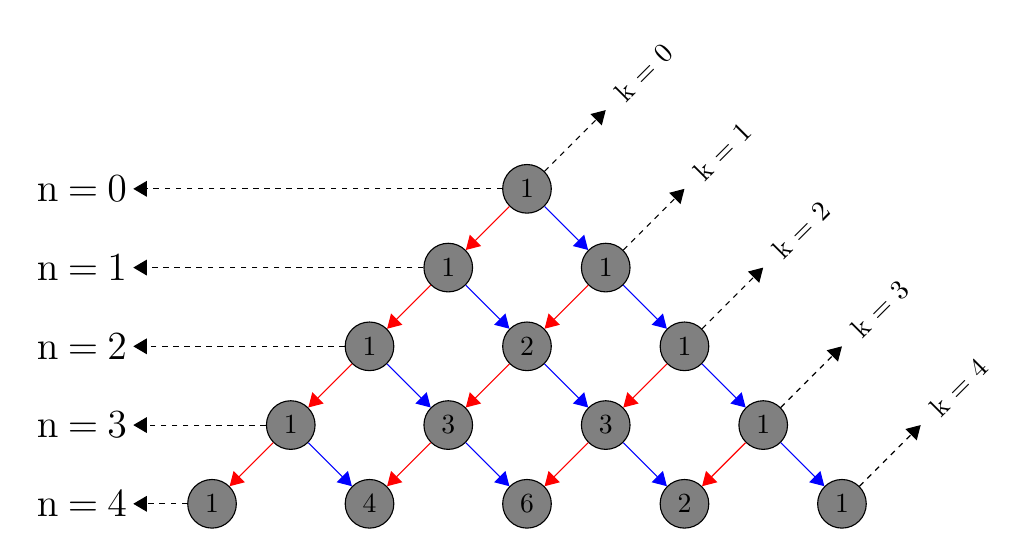
\begin{tikzpicture}

            % \draw [help lines] (0,0) grid (13,6); 

            \path   (5,4) node (a) [circle,draw,fill = gray] {1}
                    (4,3) node (b) [circle,draw,fill = gray] {1}
                    (6,3) node (c) [circle,draw,fill = gray] {1}
                    (3,2) node (d) [circle,draw,fill = gray] {1}
                    (5,2) node (e) [circle,draw,fill = gray] {2}
                    (7,2) node (f) [circle,draw,fill = gray] {1}
                    (2,1) node (g) [circle,draw,fill = gray] {1}
                    (4,1) node (h) [circle,draw,fill = gray] {3}
                    (6,1) node (i) [circle,draw,fill = gray] {3}
                    (8,1) node (j) [circle,draw,fill = gray] {1}
                    (1,0) node (k) [circle,draw,fill = gray] {1}
                    (3,0) node (l) [circle,draw,fill = gray] {4}
                    (5,0) node (m) [circle,draw,fill = gray] {6}
                    (7,0) node (n) [circle,draw,fill = gray] {2}
                    (9,0) node (o) [circle,draw,fill = gray] {1};
                
            \draw[arrows = -{Triangle[open, angle=60:2mm,fill=red]},red]  (node cs: name =a ) -- (node cs:name =b);
            \draw[arrows = -{Triangle[open, angle=60:2mm,fill=blue]},blue] (node cs: name =a ) -- (node cs:name =c);
            \draw[arrows = -{Triangle[open, angle=60:2mm,fill=red]},red] (node cs: name =b ) -- (node cs:name =d);
            \draw[arrows = -{Triangle[open, angle=60:2mm,fill=blue]},blue] (node cs: name =b ) -- (node cs:name =e);
            \draw[arrows = -{Triangle[open, angle=60:2mm,fill=red]},red] (node cs: name =d ) -- (node cs:name =g);
            \draw[arrows = -{Triangle[open, angle=60:2mm,fill=red]},red] (node cs: name =c ) -- (node cs:name =e);
            \draw[arrows = -{Triangle[open, angle=60:2mm,fill=blue]},blue] (node cs: name =c ) -- (node cs:name =f);
            \draw[arrows = -{Triangle[open, angle=60:2mm,fill=red]},red] (node cs: name =g ) -- (node cs:name =k);
            \draw[arrows = -{Triangle[open, angle=60:2mm,fill=blue]},blue] (node cs: name =g ) -- (node cs:name =l);
            \draw[arrows = -{Triangle[open, angle=60:2mm,fill=blue]},blue] (node cs: name =d ) -- (node cs:name =h);
            \draw[arrows = -{Triangle[open, angle=60:2mm,fill=red]},red] (node cs: name =h ) -- (node cs:name =l);
            \draw[arrows = -{Triangle[open, angle=60:2mm,fill=red]},red] (node cs: name =e ) -- (node cs:name =h);
            \draw[arrows = -{Triangle[open, angle=60:2mm,fill=blue]},blue] (node cs: name =h ) -- (node cs:name =m);
            \draw[arrows = -{Triangle[open, angle=60:2mm,fill=blue]},blue] (node cs: name =e ) -- (node cs:name =i);
            \draw[arrows = -{Triangle[open, angle=60:2mm,fill=red]},red] (node cs: name =i ) -- (node cs:name =m);
            \draw[arrows = -{Triangle[open, angle=60:2mm,fill=blue]},blue] (node cs: name =i ) -- (node cs:name =n);
            \draw[arrows = -{Triangle[open, angle=60:2mm,fill=red]},red] (node cs: name =f ) -- (node cs:name =i);
            \draw[arrows = -{Triangle[open, angle=60:2mm,fill=blue]},blue] (node cs: name =f ) -- (node cs:name =j);
            \draw[arrows = -{Triangle[open, angle=60:2mm,fill=red]},red] (node cs: name =j ) -- (node cs:name =n);
            \draw[arrows = -{Triangle[open, angle=60:2mm,fill=blue]},blue] (node cs: name =j ) -- (node cs:name =o);
            
            
            \draw[arrows = -{Triangle[open, angle=60:2mm,fill=black]}] [dash pattern=on 2pt off 2pt](node cs: name =a ) -- (0,4);
            \draw[arrows = -{Triangle[open, angle=60:2mm,fill=black]}] [dash pattern=on 2pt off 2pt](node cs: name =b ) -- (0,3);
            \draw[arrows = -{Triangle[open, angle=60:2mm,fill=black]}] [dash pattern=on 2pt off 2pt](node cs: name =d ) -- (0,2);
            \draw[arrows = -{Triangle[open, angle=60:2mm,fill=black]}] [dash pattern=on 2pt off 2pt](node cs: name =g ) -- (0,1);
            \draw[arrows = -{Triangle[open, angle=60:2mm,fill=black]}] [dash pattern=on 2pt off 2pt](node cs: name =k ) -- (0,0);

            \node [left=4.1cm,text width=2cm] at (a)
            {
            \mbox{\Large n = 0}
            };

            \node [left=3.1,text width=2cm] at (b)
            {
            \mbox{\Large n = 1}
            };

            \node [left=2.1,text width=2cm] at (d)
            {
            \mbox{\Large n = 2}
            };

            \node [left=1.1,text width=2cm] at (g)
            {
            \mbox{\Large n = 3}
            };

            \node [left=0.1,text width=2cm] at (k)
            {
            \mbox{\Large n = 4}
            };

            \draw[arrows = -{Triangle[open, angle=60:2mm,fill=black]}] [dash pattern=on 2pt off 2pt](node cs: name =a ) -- (6,5);
            \draw[arrows = -{Triangle[open, angle=60:2mm,fill=black]}] [dash pattern=on 2pt off 2pt](node cs: name =c ) -- (7,4);
            \draw[arrows = -{Triangle[open, angle=60:2mm,fill=black]}] [dash pattern=on 2pt off 2pt](node cs: name =f ) -- (8,3);
            \draw[arrows = -{Triangle[open, angle=60:2mm,fill=black]}] [dash pattern=on 2pt off 2pt](node cs: name =j ) -- (9,2);
            \draw[arrows = -{Triangle[open, angle=60:2mm,fill=black]}] [dash pattern=on 2pt off 2pt](node cs: name =o ) -- (10,1);
            
            \node [right=1cm,text width=1cm , rotate = 45] at (5,5)
            {
            \mbox{ k = 0}
            };

            \node [right=1cm,text width=1cm , rotate = 45] at (6,4)
            {
            \mbox{ k = 1}
            };

            \node [right=1cm,text width=1cm , rotate = 45] at (7,3)
            {
            \mbox{ k = 2}
            };

            \node [right=1cm,text width=1cm , rotate = 45] at (8,2)
            {
            \mbox{ k = 3}
            };           

            \node [right=1cm,text width=1cm , rotate = 45] at (9,1)
            {
            \mbox{ k = 4}
            };


        \end{tikzpicture}
    \end{center}

    \newpage

    \begin{center}
        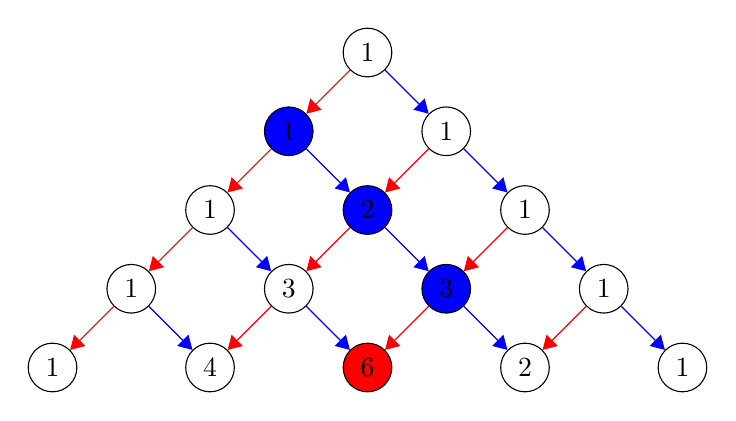
\begin{tikzpicture}

            % \draw [help lines] (0,0) grid (13,6); 

            \path   (5,4) node (a) [circle,draw,] {1}
                    (4,3) node (b) [circle,draw,fill=blue] {1}
                    (6,3) node (c) [circle,draw,] {1}
                    (3,2) node (d) [circle,draw,] {1}
                    (5,2) node (e) [circle,draw,fill=blue] {2}
                    (7,2) node (f) [circle,draw,] {1}
                    (2,1) node (g) [circle,draw,] {1}
                    (4,1) node (h) [circle,draw,] {3}
                    (6,1) node (i) [circle,draw,fill=blue] {3}
                    (8,1) node (j) [circle,draw,] {1}
                    (1,0) node (k) [circle,draw,] {1}
                    (3,0) node (l) [circle,draw,] {4}
                    (5,0) node (m) [circle,draw,fill=red] {6}
                    (7,0) node (n) [circle,draw,] {2}
                    (9,0) node (o) [circle,draw,] {1};
                
            \draw[arrows = -{Triangle[open, angle=60:2mm,fill=red]},red]  (node cs: name =a ) -- (node cs:name =b);
            \draw[arrows = -{Triangle[open, angle=60:2mm,fill=blue]},blue] (node cs: name =a ) -- (node cs:name =c);
            \draw[arrows = -{Triangle[open, angle=60:2mm,fill=red]},red] (node cs: name =b ) -- (node cs:name =d);
            \draw[arrows = -{Triangle[open, angle=60:2mm,fill=blue]},blue] (node cs: name =b ) -- (node cs:name =e);
            \draw[arrows = -{Triangle[open, angle=60:2mm,fill=red]},red] (node cs: name =d ) -- (node cs:name =g);
            \draw[arrows = -{Triangle[open, angle=60:2mm,fill=red]},red] (node cs: name =c ) -- (node cs:name =e);
            \draw[arrows = -{Triangle[open, angle=60:2mm,fill=blue]},blue] (node cs: name =c ) -- (node cs:name =f);
            \draw[arrows = -{Triangle[open, angle=60:2mm,fill=red]},red] (node cs: name =g ) -- (node cs:name =k);
            \draw[arrows = -{Triangle[open, angle=60:2mm,fill=blue]},blue] (node cs: name =g ) -- (node cs:name =l);
            \draw[arrows = -{Triangle[open, angle=60:2mm,fill=blue]},blue] (node cs: name =d ) -- (node cs:name =h);
            \draw[arrows = -{Triangle[open, angle=60:2mm,fill=red]},red] (node cs: name =h ) -- (node cs:name =l);
            \draw[arrows = -{Triangle[open, angle=60:2mm,fill=red]},red] (node cs: name =e ) -- (node cs:name =h);
            \draw[arrows = -{Triangle[open, angle=60:2mm,fill=blue]},blue] (node cs: name =h ) -- (node cs:name =m);
            \draw[arrows = -{Triangle[open, angle=60:2mm,fill=blue]},blue] (node cs: name =e ) -- (node cs:name =i);
            \draw[arrows = -{Triangle[open, angle=60:2mm,fill=red]},red] (node cs: name =i ) -- (node cs:name =m);
            \draw[arrows = -{Triangle[open, angle=60:2mm,fill=blue]},blue] (node cs: name =i ) -- (node cs:name =n);
            \draw[arrows = -{Triangle[open, angle=60:2mm,fill=red]},red] (node cs: name =f ) -- (node cs:name =i);
            \draw[arrows = -{Triangle[open, angle=60:2mm,fill=blue]},blue] (node cs: name =f ) -- (node cs:name =j);
            \draw[arrows = -{Triangle[open, angle=60:2mm,fill=red]},red] (node cs: name =j ) -- (node cs:name =n);
            \draw[arrows = -{Triangle[open, angle=60:2mm,fill=blue]},blue] (node cs: name =j ) -- (node cs:name =o);
            
            
          

           


        \end{tikzpicture}
    \end{center}

    \newpage

    \subsection*{Hockey-Stick Identity}
    \begin{center}
        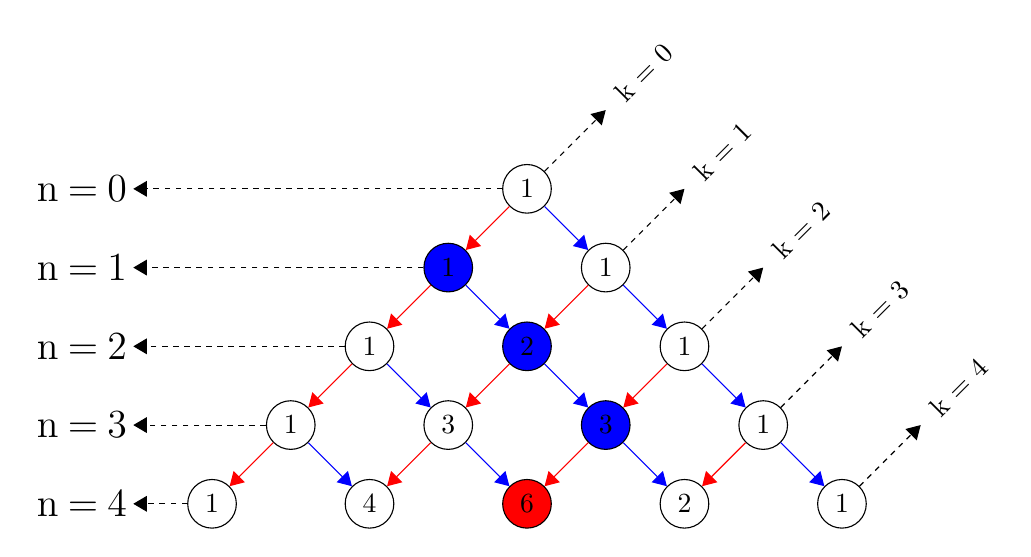
\begin{tikzpicture}

            % \draw [help lines] (0,0) grid (13,6); 

            \path   (5,4) node (a) [circle,draw,] {1}
                    (4,3) node (b) [circle,draw,fill = blue] {1}
                    (6,3) node (c) [circle,draw,] {1}
                    (3,2) node (d) [circle,draw,] {1}
                    (5,2) node (e) [circle,draw,fill = blue] {2}
                    (7,2) node (f) [circle,draw,] {1}
                    (2,1) node (g) [circle,draw,] {1}
                    (4,1) node (h) [circle,draw,] {3}
                    (6,1) node (i) [circle,draw,fill = blue] {3}
                    (8,1) node (j) [circle,draw,] {1}
                    (1,0) node (k) [circle,draw,] {1}
                    (3,0) node (l) [circle,draw,] {4}
                    (5,0) node (m) [circle,draw,fill = red] {6}
                    (7,0) node (n) [circle,draw,] {2}
                    (9,0) node (o) [circle,draw,] {1};
                
            \draw[arrows = -{Triangle[open, angle=60:2mm,fill=red]},red]  (node cs: name =a ) -- (node cs:name =b);
            \draw[arrows = -{Triangle[open, angle=60:2mm,fill=blue]},blue] (node cs: name =a ) -- (node cs:name =c);
            \draw[arrows = -{Triangle[open, angle=60:2mm,fill=red]},red] (node cs: name =b ) -- (node cs:name =d);
            \draw[arrows = -{Triangle[open, angle=60:2mm,fill=blue]},blue] (node cs: name =b ) -- (node cs:name =e);
            \draw[arrows = -{Triangle[open, angle=60:2mm,fill=red]},red] (node cs: name =d ) -- (node cs:name =g);
            \draw[arrows = -{Triangle[open, angle=60:2mm,fill=red]},red] (node cs: name =c ) -- (node cs:name =e);
            \draw[arrows = -{Triangle[open, angle=60:2mm,fill=blue]},blue] (node cs: name =c ) -- (node cs:name =f);
            \draw[arrows = -{Triangle[open, angle=60:2mm,fill=red]},red] (node cs: name =g ) -- (node cs:name =k);
            \draw[arrows = -{Triangle[open, angle=60:2mm,fill=blue]},blue] (node cs: name =g ) -- (node cs:name =l);
            \draw[arrows = -{Triangle[open, angle=60:2mm,fill=blue]},blue] (node cs: name =d ) -- (node cs:name =h);
            \draw[arrows = -{Triangle[open, angle=60:2mm,fill=red]},red] (node cs: name =h ) -- (node cs:name =l);
            \draw[arrows = -{Triangle[open, angle=60:2mm,fill=red]},red] (node cs: name =e ) -- (node cs:name =h);
            \draw[arrows = -{Triangle[open, angle=60:2mm,fill=blue]},blue] (node cs: name =h ) -- (node cs:name =m);
            \draw[arrows = -{Triangle[open, angle=60:2mm,fill=blue]},blue] (node cs: name =e ) -- (node cs:name =i);
            \draw[arrows = -{Triangle[open, angle=60:2mm,fill=red]},red] (node cs: name =i ) -- (node cs:name =m);
            \draw[arrows = -{Triangle[open, angle=60:2mm,fill=blue]},blue] (node cs: name =i ) -- (node cs:name =n);
            \draw[arrows = -{Triangle[open, angle=60:2mm,fill=red]},red] (node cs: name =f ) -- (node cs:name =i);
            \draw[arrows = -{Triangle[open, angle=60:2mm,fill=blue]},blue] (node cs: name =f ) -- (node cs:name =j);
            \draw[arrows = -{Triangle[open, angle=60:2mm,fill=red]},red] (node cs: name =j ) -- (node cs:name =n);
            \draw[arrows = -{Triangle[open, angle=60:2mm,fill=blue]},blue] (node cs: name =j ) -- (node cs:name =o);
            
            
            \draw[arrows = -{Triangle[open, angle=60:2mm,fill=black]}] [dash pattern=on 2pt off 2pt](node cs: name =a ) -- (0,4);
            \draw[arrows = -{Triangle[open, angle=60:2mm,fill=black]}] [dash pattern=on 2pt off 2pt](node cs: name =b ) -- (0,3);
            \draw[arrows = -{Triangle[open, angle=60:2mm,fill=black]}] [dash pattern=on 2pt off 2pt](node cs: name =d ) -- (0,2);
            \draw[arrows = -{Triangle[open, angle=60:2mm,fill=black]}] [dash pattern=on 2pt off 2pt](node cs: name =g ) -- (0,1);
            \draw[arrows = -{Triangle[open, angle=60:2mm,fill=black]}] [dash pattern=on 2pt off 2pt](node cs: name =k ) -- (0,0);

            \node [left=4.1cm,text width=2cm] at (a)
            {
            \mbox{\Large n = 0}
            };

            \node [left=3.1,text width=2cm] at (b)
            {
            \mbox{\Large n = 1}
            };

            \node [left=2.1,text width=2cm] at (d)
            {
            \mbox{\Large n = 2}
            };

            \node [left=1.1,text width=2cm] at (g)
            {
            \mbox{\Large n = 3}
            };

            \node [left=0.1,text width=2cm] at (k)
            {
            \mbox{\Large n = 4}
            };

            \draw[arrows = -{Triangle[open, angle=60:2mm,fill=black]}] [dash pattern=on 2pt off 2pt](node cs: name =a ) -- (6,5);
            \draw[arrows = -{Triangle[open, angle=60:2mm,fill=black]}] [dash pattern=on 2pt off 2pt](node cs: name =c ) -- (7,4);
            \draw[arrows = -{Triangle[open, angle=60:2mm,fill=black]}] [dash pattern=on 2pt off 2pt](node cs: name =f ) -- (8,3);
            \draw[arrows = -{Triangle[open, angle=60:2mm,fill=black]}] [dash pattern=on 2pt off 2pt](node cs: name =j ) -- (9,2);
            \draw[arrows = -{Triangle[open, angle=60:2mm,fill=black]}] [dash pattern=on 2pt off 2pt](node cs: name =o ) -- (10,1);
            
            \node [right=1cm,text width=1cm , rotate = 45] at (5,5)
            {
            \mbox{ k = 0}
            };

            \node [right=1cm,text width=1cm , rotate = 45] at (6,4)
            {
            \mbox{ k = 1}
            };

            \node [right=1cm,text width=1cm , rotate = 45] at (7,3)
            {
            \mbox{ k = 2}
            };

            \node [right=1cm,text width=1cm , rotate = 45] at (8,2)
            {
            \mbox{ k = 3}
            };           

            \node [right=1cm,text width=1cm , rotate = 45] at (9,1)
            {
            \mbox{ k = 4}
            };


        \end{tikzpicture}
    \end{center}


\end{document}